A model written using a modeling language like Alloy is useful to better understand the problem. In particular, it is beneficial to check if the modeling of the problem is correct or needs to be refined. Alloy generates some instances starting from the model code in order to catch modeling errors. Fixing these errors in the early stages of the system lifecycle will be significantly cheaper than fixing them at later stages of the development cycle.

\subsection{Goals of the model}
The Alloy model proposed in the next subsection of this document will focus on the formalization of the customers queueing and the slot booking system. This model is static, meaning that each instance generated by the alloy engine depicts the state of the system at a specific time instant. The goal of a static model is to generate instances of that model: these represent only the states that the system can assume. The transition between these states are instead described by a dynamic model. Finding an invalid state means that something is wrong in the system or in the model; however even if all states analyzed are correct this does not necessarily mean that the system static model is also correct.
\subsection{Alloy Code}

\lstinputlisting[language=alloy]{alloy/model.als}
\clearpage
\subsection{Instance Analysis}
In this section some generated instances by the alloy engine are shown in order to better explain the model.
For clarity some atoms and some relations between them are hidden.
\begin{figure}[H]
    \hspace*{3.0cm}
    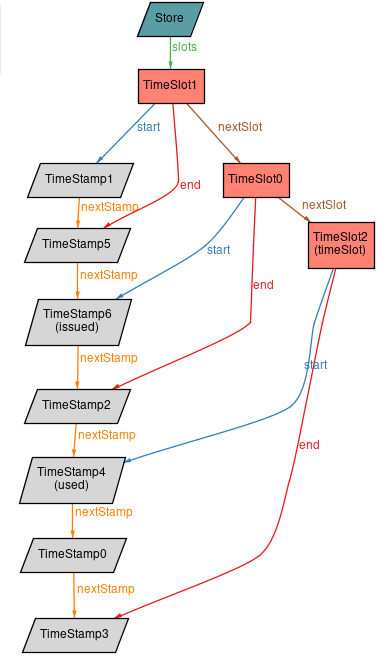
\includegraphics[scale=0.9]{Images/alloy_1_slots.png}
    \caption{\label{fig:Alloy_1}Instance diagram showing the Time Slots}
\end{figure}

As shown in Figure~\ref{fig:Alloy_1} the continuos time is modeled using discrete, ordered timestamps. A timestamp is an instant of time when something relevant for the system happens (i.e. a time slot starts, a ticket is issued or used to enter the store). Each instance offers a view of a valid system state at the last (largest) timestamp, which is \textbf{TimeStamp3} in Figure~\ref{fig:Alloy_1}.

% \pagebreak

In this instance diagram, time slots atoms are shown. Every couple of TimeSlots created by the same store must not overlap and the next TimeSlot should start after the end of the current one.

\vfill
\pagebreak

\begin{figure}[H]
    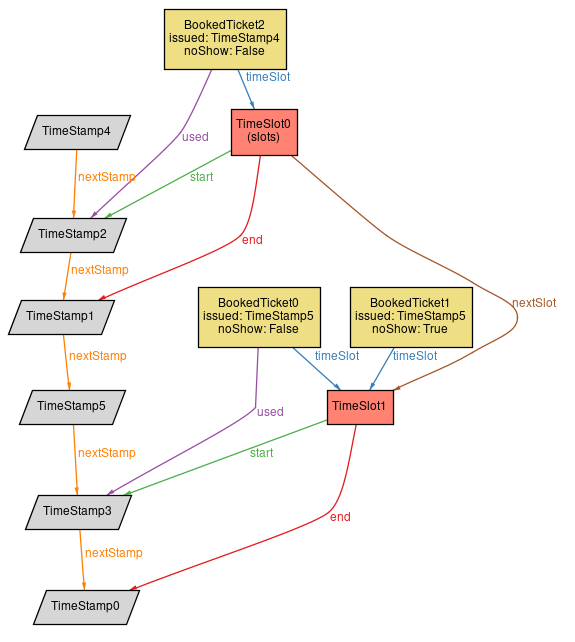
\includegraphics[width=\textwidth]{Images/alloy_3_booked.png}
    \caption{\label{fig:Alloy_2}Instance diagram showing Booked Tickets}
\end{figure}
In Figure~\ref{fig:Alloy_2} booked tickets are shown in the diagram. BookedTickets are a special type of ticket that is bound to a TimeSlot. A Booked Ticket must be issued before the start of the time slot, and it has to be used within its associated TimeSlot. A BookedTicket not used in its TimeSlots counts as a \textbf{no-show} ticket (which represents a customer that books a ticket but does not show up to the store in time).

\vfill
\pagebreak

\begin{figure}[H]
    \hspace*{2.8cm}
    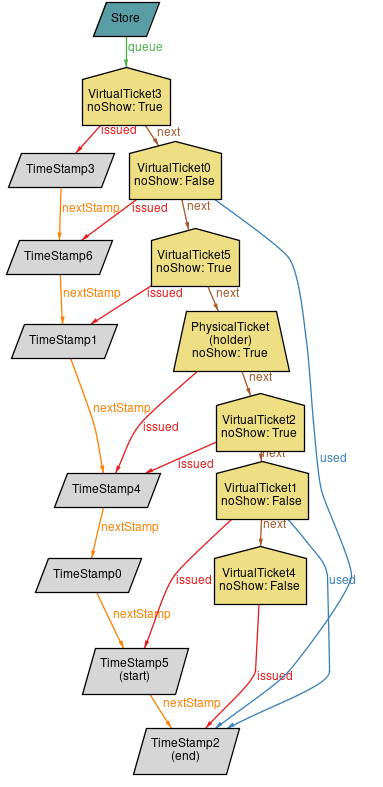
\includegraphics[scale=0.9]{Images/alloy_2_queue.png}
    \caption{\label{fig:Alloy_3}Instance diagram showing the queueing system}
\end{figure}

The Figure~\ref{fig:Alloy_3} explains how the store queueing system is modeled. If a customer doesn't book a ticket to enter the store, they have to retrieve a NumberedTicket, either Virtual (using the application) or Physical (using the ticket emitter). These tickets are handed using a \textbf{First Come First Served} Logic: a ticket with a lower TimeStamp should be called to the entrance before a ticket with an higher one. The TimeStamp representing when the ticket is used should also reflect this order unless no-shows happen (i.e. A customer that retrieves a ticket and then does not show when called to the entrance).